% ----------------------------------------

\subsection{Overview}

% ----------------------------------------

\begin{frame}

\frametitle{Assumptions}
\framesubtitle{E-commerce website}

For this project, we are required to design an \textbf{Environment} that satisfies various constraints both on the e-commerce site's properties and on the users' behavior; in addition, since most of the tasks were generic, we had to come up with some of our own assumptions.

In particular we want to underline the following assumptions for the e-commerce website:
\begin{itemize}[label={-}]
    \item The website has unlimited stock for the 5 different items.
    \item Actions on the various webpages are \textbf{perfectly observable} by the e-commerce website.
\end{itemize}

\end{frame}

% ----------------------------------------

\begin{frame}

\frametitle{Assumptions}
\framesubtitle{Users}

...and we assume that the users present the following behaviors:
\begin{itemize}[label={-}]
    \item Every day, there is a random number (subject to noise) of potential new users.
    \item The users can activate \textbf{parallel paths} while on the website.
    \item The number of items that a user will buy is a random variable, independent from any other variable; but every user that lands on the page of a product will buy at least 1 unit of it if it's under their \textbf{reservation price}.
    \item The behavior of users can be modelled as a graph where \textit{nodes} represent product pages and \textit{weights} represent the probabilities for a user to click from the primary item of the page to one of the secondaries.
\end{itemize}

\end{frame}

% ----------------------------------------

\subsection{Environment structure}

% ----------------------------------------

\begin{frame}[fragile]

\frametitle{Environment}
\framesubtitle{Structure}

The environment is modelled as a python dataclass containing the following attributes:

\begin{lstlisting}[style=Python, basicstyle=\tiny, numbers=none, framexrightmargin=-20pt]
    # The total budget to subdivide
    total_budget: int

    # Probability of every class to show up. They must add up to 1
    class_ratios: List[float]

    # Features associated to every class
    class_features: List[List]

    # Price of the 5 products
    product_prices: List[float]

    # List of class parameters for each class and product,
    # implemented as list of lists of UserClassParameters.
    # Each class has distinct parameters for every product
    classes_parameters: List[List[UserClassParameters]]
\end{lstlisting}

\end{frame}

% ----------------------------------------

\begin{frame}[fragile]

\frametitle{Environment}
\framesubtitle{Structure}

\begin{lstlisting}[style=Python, basicstyle=\tiny, numbers=none, framexrightmargin=-20pt]
    # Lambda parameter, which is the probability of osserving the
    # next secondary product according to the project's assignment
    lam: float

    # Max number of items a customer can buy of a certain product.
    # The number of bought items is determined randomly with
    # max_items as upper bound
    max_items: int

    # Products graph's matrix. It's a empty matrix, should be
    # initialized with populate_graphs
    graph: np.ndarray

    # List that constains for every i+1 product the secondary i+1
    # products that will be shown in the first and second slot
    next_products: List[Tuple[int, int]]

    # Controls randomness of the environment
    random_noise: float
\end{lstlisting}

\end{frame}

% ----------------------------------------

\begin{frame}

\frametitle{Environment}
\framesubtitle{Masked Environment}

Alongside the \textbf{Environment} we define a \textbf{Masked Environment} with the purpose of \textit{hiding crucial information} to the learners since each type of learner should only have access to a subset of all the information available in the environment dictated by the type of learner.

The masked environment isn't strictly needed in the project since the learners could easily ignore the extra information, however, we wanted to face the problem with an approach aimed towards reusability and extendability and in this case (as in many others down the line) we opted for a more \textbf{generalizable} solution.

\end{frame}

% ----------------------------------------

\begin{frame}

\frametitle{Users}
\framesubtitle{User parameters}

We modelled the $\alpha$-functions, which compute the expected value of interactions on a product given a fixed budget, as \textbf{exponential functions}.

In particular their \textit{upper bound} represents the maximum expected number of interactions possible while the \textit{maximum useful budget} is the amount of budget after which any budget increase would not lead to a ratio increase.

\end{frame}

% ----------------------------------------

\begin{frame}

\frametitle{Users}
\framesubtitle{User classes}

Users are subdivided in classes based on their \textit{2 binary features} for a total of \textit{3 different classes}.

In particular, each user class is defined by its $\alpha$-functions (one for each product plus the one for the non-strategic competitor) which define the probability of landing on a given product page.

Each $\alpha$-function is defined by the values: \textbf{reservation price}, \textbf{upper bound} and \textbf{maximum useful budget}

\end{frame}

% ----------------------------------------

\subsection{Randomness in the Environment}

% ----------------------------------------

\begin{frame}

\frametitle{Randomness in the Environment}
\framesubtitle{Non determinism}

For the sake of representing a real scenario, most of the values that are not known a priori are \textit{randomly generated} and every variable that evolves through time without our direct control has elements of randomness to it (for instance, each day we randomly get the number of active total users in our scenario by using a gaussian distribution with tunable mean and standard deviation).

Even though most of the randomness is tunable and controlled through seeded generators, there are still \textbf{impactful elements of non determinism} (i.e. the Dirichlet distribution) that are not possible to control in any way.

\end{frame}

% ----------------------------------------

\subsection{Simulation}

% ----------------------------------------

\begin{frame}

\frametitle{Daily Simulation}
\framesubtitle{Purpose}

The \textbf{Simulation} class is the main engine that brings together \textit{learners} and \textit{environment} by making them interact with each other while offering an interface to customize the execution.

The basic idea of the simulation is to simulate a real scenario day by day using the environment to generate interactions with the website according to the budgets that the current learner proposed and then, feed the results back to the learner to make it actually learn.

Repeating the simulation execution step for each day until an arbitrary \textbf{time horizon} is reached grants us all the data needed to evaluate the performance of our learner.

\end{frame}

% ----------------------------------------

\begin{frame}

\frametitle{Daily Simulation}
\framesubtitle{Example}

\scriptsize
Simulation runs of two learners with having an environment with total\_budget = 400 and population\_mean = 1000

\begin{center}
    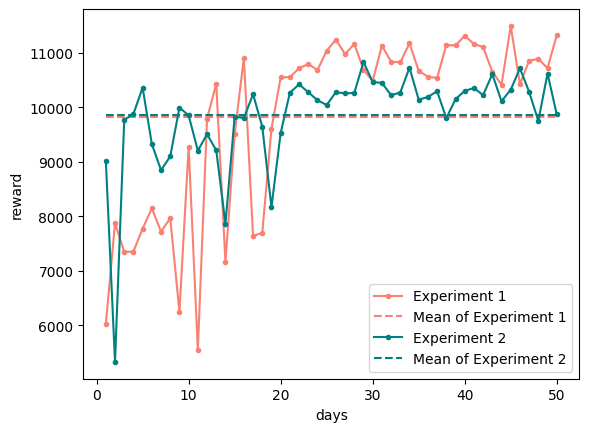
\includegraphics[scale=0.5]{img/Graphs/env_sim/image1.png}
\end{center}


\end{frame}

% ----------------------------------------
